\section{Aurushire}

Aurushire (also commonly referred to as Goldshire) is a small village located on the southern end of the Statu peninsula. Just East of Aurushire is a large mountain containing mine shafts used for gold mining. It is not well known, other by those who work in the mines, but strange things happen within these mines where mined gold will spontaneously be regrown after being removed from the mines. This phenomenon is where Aurushire (Goldshire) retreived its name from and is thought to be related to the spacial occurrences reported in The Pluvian Forest. 

\begin{center}
	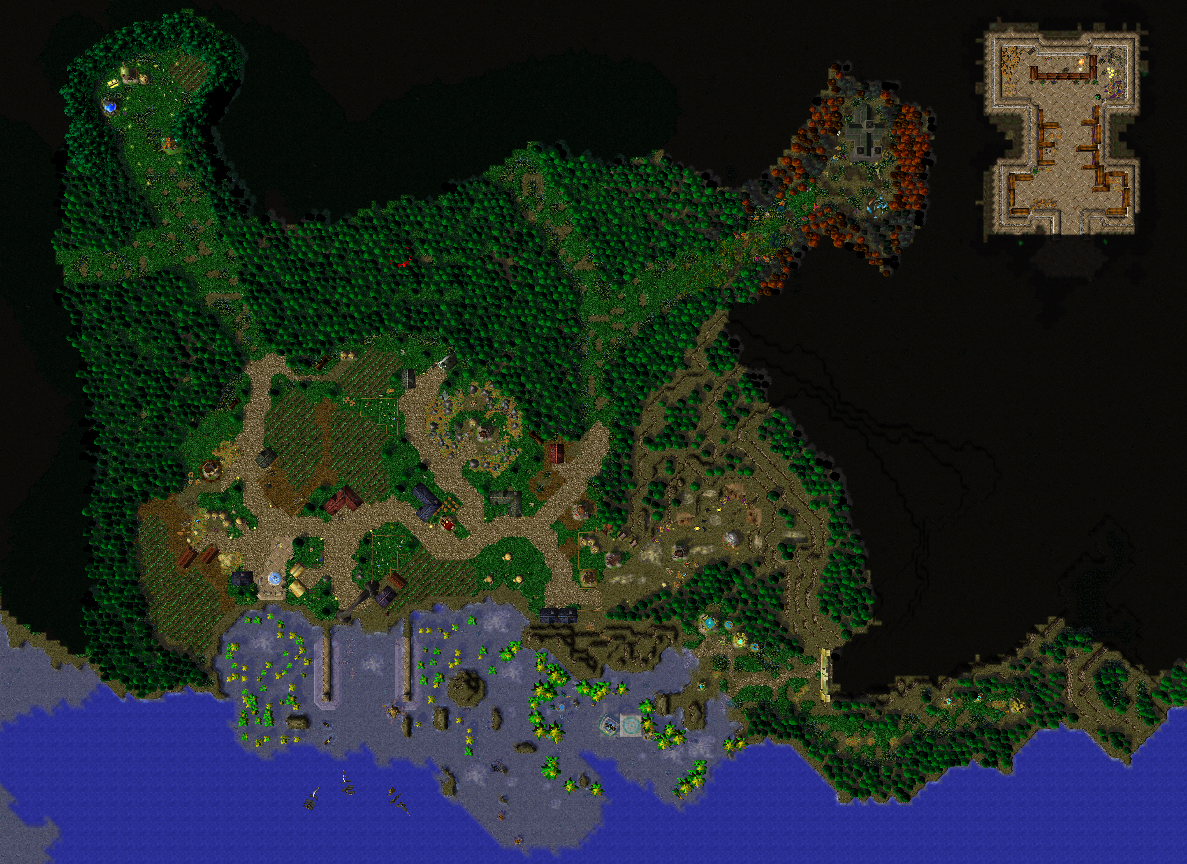
\includegraphics[width=\linewidth]{img/maps/Aurushire.png}
	
	{\textbf{Aurushire:} To the south is the sea entrance. In the northwest is a secluded area where Baba Lives. To the northeast is a secluded area where Belmod lives. The North path leads to The Pluvian Forest and the West path leads to Rem Silva. The East side of the village is the location of Auru Convallis and the Naga camps are on the southeast side of the area leading into the eastern forest.}
\end{center}

\subsection{NPC's}

Aurushire is full of NPC characters. Many of them are just normal workers or village folk, however some serve an important purposes. Some of them include the innkeeper, the Pandaren Brothers, the village watchers and the shopkeepers.

\begin{monsterbox}{Arryn}
	\begin{hangingpar}
		\textit{Halfling Wizard, Neutral Good}
	\end{hangingpar}
	\dndline%
	\basics[%
	armorclass = 17,
	hitpoints  = 172,
	speed      = 40 ft
	]
	\dndline%
	\stats[
	STR = \stat{12}, % This stat command will autocomplete the modifier for you
	DEX = \stat{12},
	CON = \stat{16},
	INT = \stat{20},
	WIS = \stat{18},
	CHA = \stat{18}
	]
	\dndline%
	\details[%
	% If you want to use commas in these sections, enclose the
	% description in braces.
	% I'm so sorry.
	languages = {Common, Elvish, Dwarvish, Gnomish, Halfling, Orc, Pandaren},
	challenge = 10
	]
	\dndline%
	\begin{monsteraction}[Mystical Senses]
		If a target tries to deceive you, it must make a DC19 deception saving throw.
	\end{monsteraction}	
	\begin{monsteraction}[Water sight]
		You can see clearly up to two miles over water.
	\end{monsteraction}
	\monstersection{Actions}
	\begin{monsteraction}[Bladesinger: Extra Attack]
		You can attack twice on your turn.
	\end{monsteraction}
	\begin{monsteraction}[Hold Monster]
		A creature you can see within 90 feet must succeed on a wisdom saving throw or be paralyzed for 1 minute. Target can make a wisdom saving throw at the end of each of it's turns to end the spell.
	\end{monsteraction}
	\begin{monsteraction}[Magic Jar Master]
		Allows Arryn to use Magic Jar on a nearby jar instantly and without being in a jar himself.
	\end{monsteraction}
	\begin{monsteraction}[Magic Jar]
		Long description, look it up.
	\end{monsteraction}
	\monstersection{Description/Information}
	Arryn is the first NPC most encounter when entering Aurushire from sea. He is the watcher of the ports and lives on a small farm right at docks where all sea traffic enters from.
\end{monsterbox}

\begin{monsterbox}{Tamina}
	\begin{hangingpar}
		\textit{Human Ranger, Neutral Good}
	\end{hangingpar}
	\dndline%
	\basics[%
	armorclass = 18,
	hitpoints  = 154,
	speed      = 40 ft
	]
	\dndline%
	\stats[
	STR = \stat{18}, % This stat command will autocomplete the modifier for you
	DEX = \stat{18},
	CON = \stat{12},
	INT = \stat{14},
	WIS = \stat{13},
	CHA = \stat{11}
	]
	\dndline%
	\details[%
	% If you want to use commas in these sections, enclose the
	% description in braces.
	% I'm so sorry.
	languages = {Common, Elvish, Pandaren},
	challenge = 10
	]
	\dndline%
	\begin{monsteraction}[Mystical Senses]
		If a target tries to deceive you, it must make a DC19 deception saving throw.
	\end{monsteraction}	
	\begin{monsteraction}[Water sight]
		You can see clearly up to two miles over water.
	\end{monsteraction}
	\begin{monsteraction}[Bladesinger: Extra Attack]
		You can attack twice on your turn.
	\end{monsteraction}
	\monstersection{Actions}
	\begin{monsteraction}[Paralytic Dart]
		Hit: +3. A creature you can see within 90 feet must succeed on a wisdom saving throw or be paralyzed for 1 minute.
	\end{monsteraction}
	\begin{monsteraction}[Aimed Shot]
		Hit: +6. Damage: 3d6 + 4 piercing damage. You pull our your longbow and fire a single arrow aimed precisely where you choose. 
	\end{monsteraction}
	\begin{monsteraction}[Scatter Shot]
		Hit: +6. Damage 1d6 + 2 piercing damage per arrow. You grasp up to 4 arrows and mount them in your bow. You must roll hit for each arrow you attempt to fire and can choose up to 4 targets for the various arrows.
	\end{monsteraction}
	\begin{monsteraction}[Blade Slash]
		Hit: +5. Damage 2d6 + 3 slashing damage per arrow. You pull our your silvered short sword and make a melee attack against the target.
	\end{monsteraction}

	\monstersection{Description/Information}
	Tamina is a watcher of Aurushire. She trains under Arryn and the Stormstout brothers and spends the majority of her time roaming the outskirts of the town keeping watch for dangers or new occurrences in the area.
\end{monsterbox}

\begin{center}
	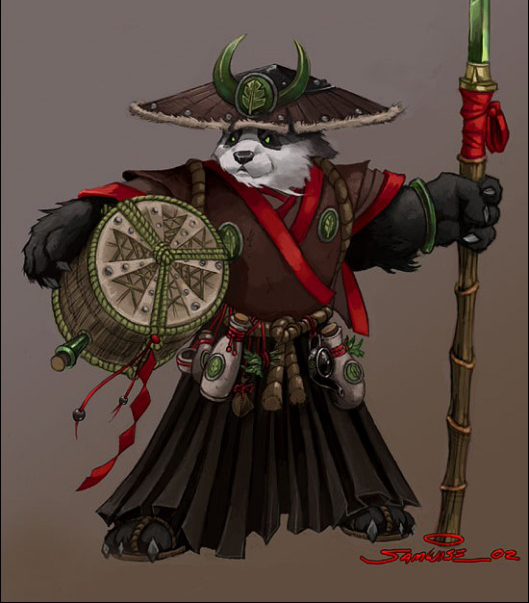
\includegraphics[width=0.39\linewidth]{img/WoW/chen.jpg} 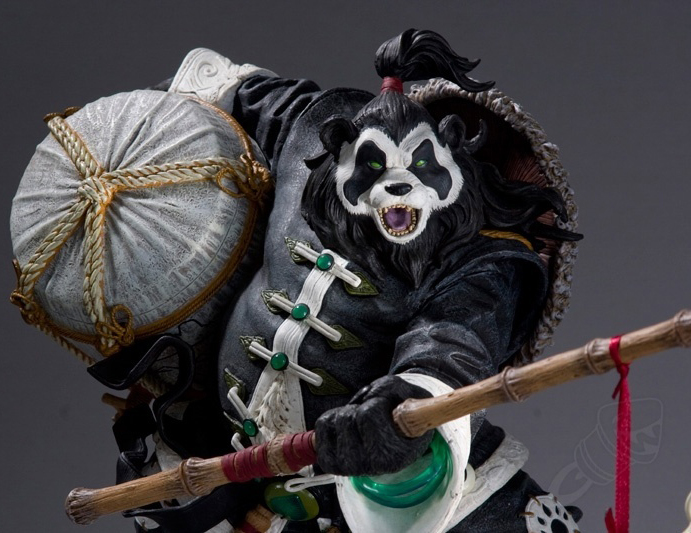
\includegraphics[width=0.575\linewidth]{img/WoW/153930.jpg}
\end{center}

\begin{monsterbox}{Chen Stormstout}
	\begin{hangingpar}
		\textit{Pandaren Monk, Neutral Good}
	\end{hangingpar}
	\dndline%
	\basics[%
	armorclass = 17,
	hitpoints  = 172,
	speed      = 40 ft
	]
	\dndline%
	\stats[
	STR = \stat{18}, % This stat command will autocomplete the modifier for you
	DEX = \stat{20},
	CON = \stat{16},
	INT = \stat{12},
	WIS = \stat{12},
	CHA = \stat{18}
	]
	\dndline%
	\details[%
	% If you want to use commas in these sections, enclose the
	% description in braces.
	% I'm so sorry.
	languages = {Common, Elvish, Dwarvish, Gnomish, Halfling, Orc, Pandaren},
	challenge = 10
	]
	\dndline%
	\begin{monsteraction}[Joint lock]
		You can put a creature in a joint lock when attacking. Remove 1d6 damage from the attack and instead roll 1d20 to decide on how severe the joint lock is. 
		
		1-3: The joint lock fails. 
		
		4-14: You pop a joint briefly out of place causing the enemy to have disadvantage on their next attack.
		
		15-19: You dislocate the targeted limb, causing the opponent to not be able to use it until set (which can be done via an action on their turn). You can choose to roll less if desired.
		
		20: You tear the tendons holding a limb on, causing it to become useless until healed. You can choose to roll less if desired.
	\end{monsteraction}
	\begin{monsteraction}[Pressure Point Mastery]
		You can target a creatures pressure points when attacking. Remove 1d6 damage from the attack and instead roll 1d20 to decide how accurate the points are hit. 
		
		1-3: The pressure points fail. 
		
		4-14: You hit a target in a precious spot causing them great discomfort. They must roll attack rolls at disadvantage next round.
		
		15-19: The target becomes stunned for one round of combat. You can choose to roll less if desired.
		
		20: The target becomes completely paralyzed. You can choose to roll less if desired.
	\end{monsteraction}
	\monstersection{Actions}
	\begin{monsteraction}[Pandaren Nimbleness: Extra Attack]
		You can attack twice on your turn.
	\end{monsteraction}
	\begin{monsteraction}[Melee]
	This is a normal un-armed melee attack: +6 to hit. Deals 3d6 +5 damage.
	\end{monsteraction}
	\begin{monsteraction}[Armed Melee]
		This is a normal melee attack using a weapon. Depending on the weapon, it can add damage to the Melee attack. Spear/staff: +6 damage, Sword: +4 damage, Hammer/Axe: +2 damage.
	\end{monsteraction}

	\monstersection{Description/Information}
	Chen Stormstout runs the Aurushire Pub. He spends his time wandering the nearby regions for herbs and ingredients to make the perfect brews. He also studies martial arts with his brothers. He focuses on pressure points and joint locks and studies a more fluid form of combat.
\end{monsterbox}

\begin{center}
	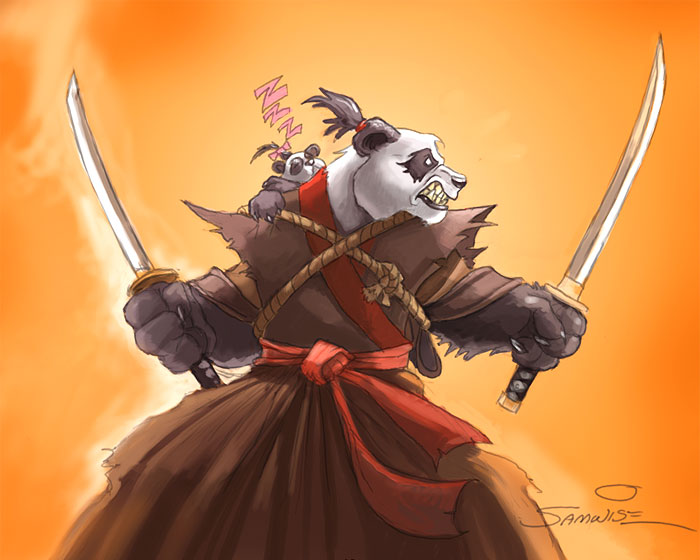
\includegraphics[width=0.60\linewidth]{img/WoW/ekron.jpg} 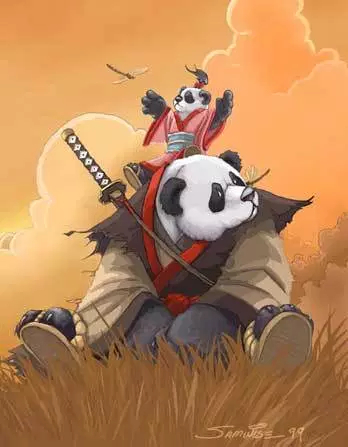
\includegraphics[width=0.375\linewidth]{img/WoW/twopandare.jpg}
\end{center}

\begin{monsterbox}{Ekron Stormstout}
	\begin{hangingpar}
		\textit{Pandaren Barbarian, Neutral Good}
	\end{hangingpar}
	\dndline%
	\basics[%
	armorclass = 17,
	hitpoints  = 172,
	speed      = 50 ft
	]
	\dndline%
	\stats[
	STR = \stat{20}, % This stat command will autocomplete the modifier for you
	DEX = \stat{18},
	CON = \stat{18},
	INT = \stat{12},
	WIS = \stat{12},
	CHA = \stat{16}
	]
	\dndline%
	\details[%
	% If you want to use commas in these sections, enclose the
	% description in braces.
	% I'm so sorry.
	languages = {Common, Elvish, Dwarvish, Gnomish, Halfling, Orc, Pandaren},
	challenge = 10
	]
	\dndline%
	\begin{monsteraction}[Fury of Blows]
		If you have two swords, you can furiously attack your opponent without them being able to block. You can sacrifice any number of 1d6's from the attack roll to destroy an item the opponent has on them.
	\end{monsteraction}	
	\monstersection{Actions}
	\begin{monsteraction}[Pandaren Nimbleness: Extra Attack]
		You can attack twice on your turn.
	\end{monsteraction}
	\begin{monsteraction}[Melee]
	This is a normal un-armed melee attack: +6 to hit. Deals 3d6 +5 damage.
	\end{monsteraction}
	\begin{monsteraction}[Armed Melee]
		This is a normal melee attack using a weapon. Depending on the weapon, it can add damage to the Melee attack. Spear/staff: +4 damage, Sword: +6 damage, Hammer/Axe: +2 damage.
	\end{monsteraction}
	\monstersection{Description/Information}
	Ekron, like his brothers, also studies martial arts.He focuses on agility and movements to quickly take down his opponents with a fierce and fast form of combat. He is the keeper of the Aurushire Quarries and leads the mining operations. He found a small panda in the forest one day and has been cherishing it ever since as a friend and companion.
\end{monsterbox}

\begin{center}
	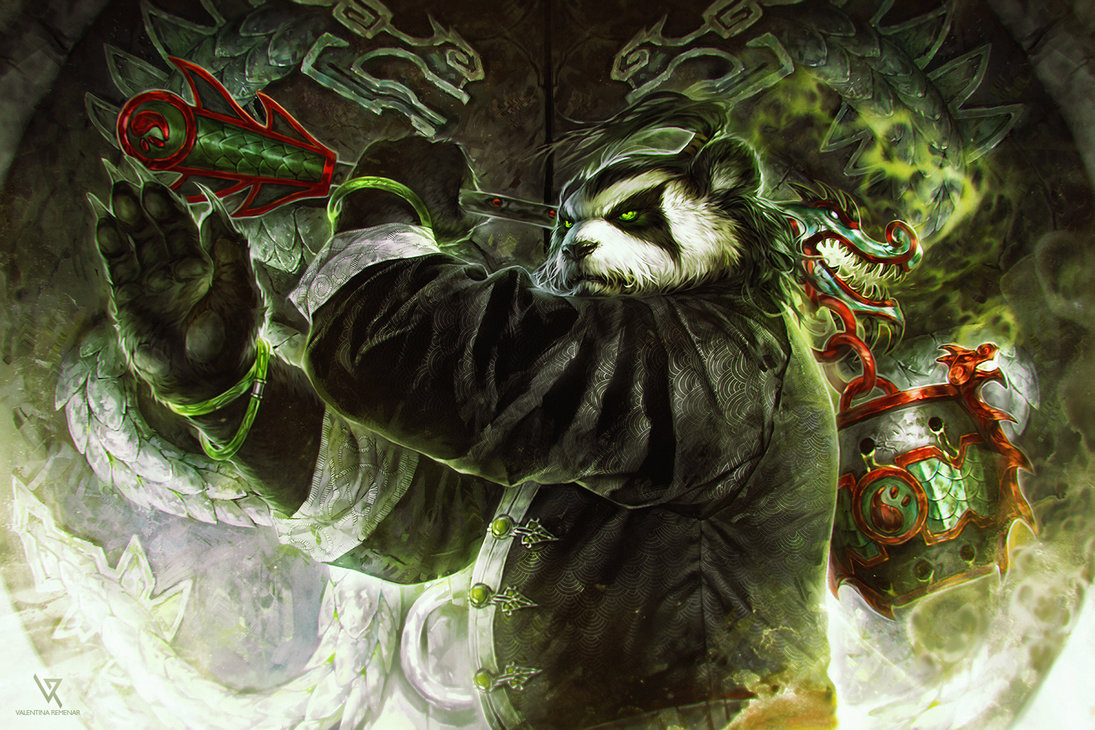
\includegraphics[width=0.48\linewidth]{img/WoW/mishnah.jpg} 		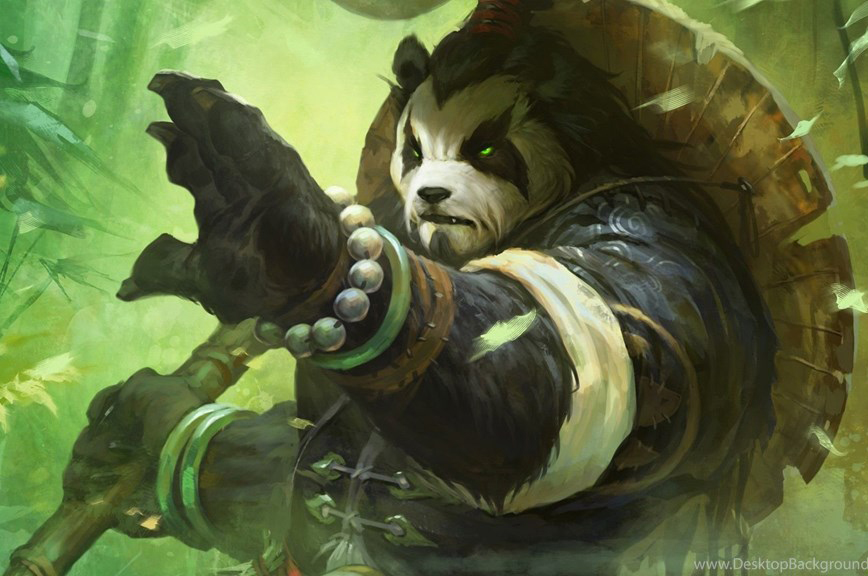
\includegraphics[width=0.48\linewidth]{img/WoW/mishna.jpg}
\end{center}

\begin{monsterbox}{Mishnah Stormstout}
	\begin{hangingpar}
		\textit{Pandaren, Neutral Good}
	\end{hangingpar}
	\dndline%
	\basics[%
	armorclass = 17,
	hitpoints  = 172,
	speed      = 30 ft
	]
	\dndline%
	\stats[
	STR = \stat{20}, % This stat command will autocomplete the modifier for you
	DEX = \stat{18},
	CON = \stat{18},
	INT = \stat{12},
	WIS = \stat{16},
	CHA = \stat{18}
	]
	\dndline%
	\details[%
	% If you want to use commas in these sections, enclose the
	% description in braces.
	% I'm so sorry.
	languages = {Common, Elvish, Dwarvish, Gnomish, Halfling, Orc, Pandaren},
	challenge = 10
	]
	\dndline%
	\begin{monsteraction}[Thunderous Blow]
		You can sacrifice 2d6 on an attack roll to instead deal 1d4 thunderous damage to all enemies within 15 feet of the blow you deal.
	\end{monsteraction}	
	\monstersection{Actions}
	\begin{monsteraction}[Pandaren Nimbleness: Extra Attack]
		You can attack twice on your turn.
	\end{monsteraction}
	\begin{monsteraction}[Melee]
		This is a normal un-armed melee attack: +6 to hit. Deals 3d6 +5 damage.
	\end{monsteraction}
	\begin{monsteraction}[Armed Melee]
		This is a normal melee attack using a weapon. Depending on the weapon, it can add damage to the Melee attack. Spear/staff: +2 damage, Sword: +4 damage, Hammer/Axe: +6 damage.
	\end{monsteraction}
	\monstersection{Description/Information}
	Mishnah Stormstout is the Aurushire Blacksmith. He spends his time collecting rocks and forging precious metals found in his brothers mine. He also studies martial arts but tends more towards a body building focus and overpowers his foes through brute strength.
\end{monsterbox}

\begin{center}
	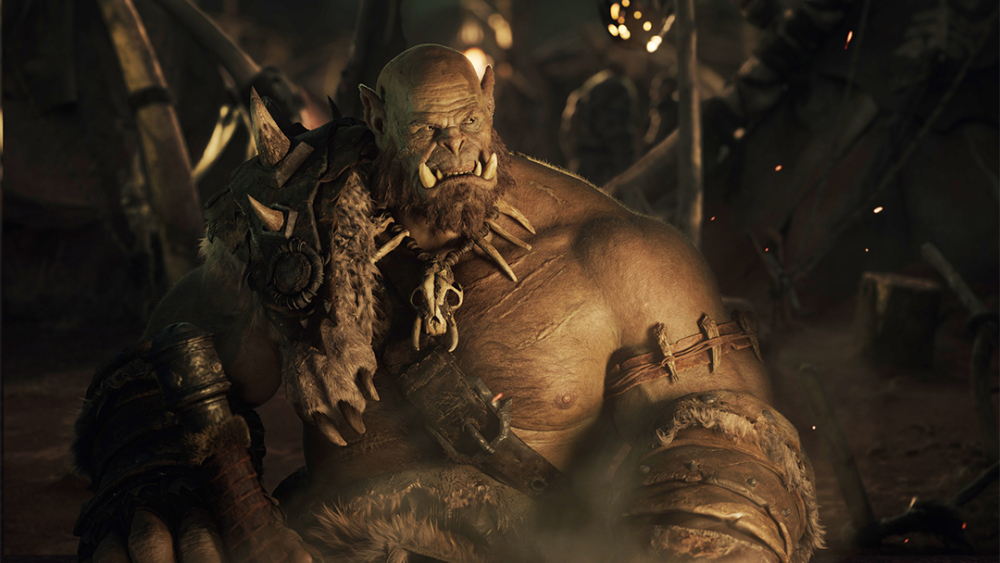
\includegraphics[width=0.7\linewidth]{img/WoW/bob.jpg}
\end{center}

\begin{monsterbox}{Bob}
	\begin{hangingpar}
		\textit{Orcish Barbarian, Neutral Good}
	\end{hangingpar}
	\dndline%
	\basics[%
	armorclass = 17,
	hitpoints  = 151,
	speed      = 30 ft
	]
	\dndline%
	\stats[
	STR = \stat{20}, % This stat command will autocomplete the modifier for you
	DEX = \stat{18},
	CON = \stat{17},
	INT = \stat{16},
	WIS = \stat{15},
	CHA = \stat{13}
	]
	\dndline%
	\details[%
	% If you want to use commas in these sections, enclose the
	% description in braces.
	% I'm so sorry.
	languages = {Common, Dwarvish, Orc},
	challenge = 9
	]
	\dndline%
	\begin{monsteraction}[Experienced Pain]
		Bob has seen some things. He can ignore any major wounds or hindrances that would effect his combat. He can fight full power until his last breath. This is due to his combat experience and many near death experiences.
	\end{monsteraction}	
	\begin{monsteraction}[Battle Master]
		Bob can quickly pick up and adapt to using most weapons, gaining proficiency with any new weapons after using them.
	\end{monsteraction}	
	\monstersection{Actions}
	\begin{monsteraction}[Combat experience: Extra Attack]
		You can attack twice on your turn.
	\end{monsteraction}
	\begin{monsteraction}[Melee]
		This is a normal un-armed melee attack: +6 to hit. Deals 2d6 +5 damage.
	\end{monsteraction}
	\begin{monsteraction}[Throwing Axe]
		Bob carries 4 throwing axes that he can hurl towards an enemy. +5 to hit. 3d6 +2 damage. Range: 40 ft.
	\end{monsteraction}
	\monstersection{Description/Information}
	
\end{monsterbox}


\subsection{The Inn of the Prancing Pony}

This is the inn located in Aurushire. The innkeeper is named Artemisia who is kind of like the grandmother of the small village. 

\subsection{Tracey's Armory}

Tracey's Armory is the armor shop in Aurushire. The shopkeeper is Tiberias Tracey, who is one of the great grandchildren of the original shop's builder. This shop contains simple and custom armor pieces that are created for all who are willing to pay or friends of Tiberias. 

\subsection{Bob's Guns}

Bob's Guns is a relatively newly built shop. The majority of what is sold here is ranged weapons. Due to the effects of the Pluvian Forest, Bob (the storekeeper) discovered a weapon laying in the wild on someones corpse. He was able t reverse engineer approximately how it worked and has been creating 'guns' ever since. Unfortunately he used all of the bullets on the original design, but he was able to examine the weapon itself and deduce a process to recreate a similar mechanism, His own designs are not as well made as the original discovery, but they are slowly improving over time. Bob also sells spears, throwing stars, darts, bows and more.

\subsection{Stormstout Blacksmith}

This is the village blacksmith that is run by one of the Stormstout brothers (Mishnah). The blacksmith is one of the watchers of the village and most influential members. Mishnah is also friends with everyone else in the village and generally his services are needed by almost all of the members.

\begin{commentbox}{Working in the Mines}
	The players are able to work in the blacksmith for either gold or skills. The players can work for either 20 gold a day or they can work for one of the following skills.
	\begin{description}
		\item[7 day:] Apprentice smithy: They can be taught how to make basic smithing items. Their success on the items will depend on a d20 roll.
		\item[1 month:] Novice smithy: They can be taught how to make novice smithing items and possibly enhance other items. Their success on the items will depend on a d20 roll.
		\item[1 year:] Master smithy: They can be taught how to make master smithing items and enhance other smithed items. Their success on the items will depend on a d20 roll.
	\end{description}
\end{commentbox}

\subsection{Stormstout Pub}

This is the village brewery which is unlike any brewery anywhere else. The brewery is run by one of the Stormstout brothers (Chen). Chen ha ssome of the most unique brews of anywhere else in Orilla. This is primarily due to the ingredients and herbs that he has found throughout the nearby forests. Chen is one of the friendliest people in Aurushire and most people go to him with their issues or thoughts. He is generally a sociable person and many people hang out at his Brewery/Pub in their free time. Chen is also one of the watchers of the village and most influential members.

\begin{commentbox}{Working in the Mines}
	The players are able to work in the pub for either gold or skills. The players can work for either 20 gold a day or they can work for one of the following skills.
	\begin{description}
		\item[7 day:] Apprentice brewer: They can be taught how to make brews from new ingredients they find. Their success on the brews will depend on a d20 roll.
		\item[1 month:] Novice brewer: They can be taught how to make Novice brews and potions from new ingredients they find. Their success on the brews will depend on a d20 roll.
		\item[1 year:] Master brewer: They can be taught how to make master brews, potions, and elixirs from new ingredients they find. Their success on the brews will depend on a d20 roll.
	\end{description}
\end{commentbox}

\subsection{Stormstout Quarries}

The Stormstout Quarries are the mines that reside to the East of Aurushire. The mines are run by one of the Stormstout brothers (Ekron). Ekron is a strong military leader and one of the most influential members of Aurushire. The mines are known for their unique regrowth of some of the ores within them. It is believed that these occurrences are as a result of effects on the region by the Pluvian Forest. The quarries will pay any willing workers with a part of their earnings. Ekron is one of the watchers of the village.

\begin{commentbox}{Working in the Mines}
	The players are able to work in the mines for gold. The payout for gold is dealt daily and events occurring in the mines can be determined by rolling a d20. The mines are generally safe, but can be dangerous if you are not paying attention. Before working in the mines the players must agree to the terms of work which include replacing equipment destroyed by their use.
	
	\begin{description}
		\item[1:] Disaster struck while you were in the mine. You end up fracturing a limb (making it un-usable until healed) and breaking some equipment that you rented. You have to repay for the equipment which totals 300g. If the player does not have this they go in debt.
		\item[2:] Disaster struck while you were in the mine. breaking some equipment that you rented. You have to repay for the equipment which totals 300g. If the player does not have this they go in debt.
		\item[3:] Disaster struck while you were in the mine. breaking some equipment that you rented. You have to repay for the equipment which totals 100g. If the player does not have this they go in debt.
		\item[4:] You were unable to make much progress in the mine. You're tired, exhausted, and have not come out with any profits. You only have to pay a renting fee for the equipment you borrowed which totals 10g. If the player does not have this they go in debt.
		\item[5-6:] You have a sluggish day in the mine. You break even walking away with no profit.
		\item[7-10:] You worked a descent shift. You struck gold (literally) and tried to mine it all well. Your cut for the day is 10g.
		\item[11-14:] You worked a descent shift. You struck gold (literally) and tried to mine it all well. Your cut for the day is 25g.
		\item[15-16:] You worked a great shift. You struck gold (literally) mined it all well. Your cut for the day is 50g.
		\item[17:] You worked a great shift. You struck gold (literally) mined it all well. Your cut for the day is 100g.
		\item[18:] You worked a perfect shift. You struck gold (literally) mined it all perfectly. Your cut for the day is 200g.
		\item[19:] You worked a perfect shift. You struck gold (literally) mined it all perfectly. Your cut for the day is 400g.
		\item[20:] You worked a perfect shift. You struck gold (literally) and also stumbled across a new rare gemstone and mined it all perfectly. Your cut for the day is 1000g.
	\end{description}
\end{commentbox}

\subsection{Library of Lysanias}

The village has a library that is open to all. There are a number of people who spend a lot of time here and maintain it but for the most part it is open and there is no main keeper. The library is public and contains mostly learning material and books written by previous and past villagers.